\subsubsection{Pricing American Options by Randomized Quasi-Monte Carlo}
Options are the opportunity to purchase or sell an asset (stock) at a fixed price some time in the
future. 
The payoff of an option depends on the path that the stock price takes. 
Asset prices are often described for continuous time, i.e., $t > 0.$ Here, we use the geometric Brownian
motion model:
$S(t) = S(0) \exp((r - \sigma^2/2)t + \sigma B(t)), t \ge 0,$
where $B(\cdot )$ is a standard Brownian motion (BM) and $\sigma$ is the volatility of the asset. To get the payoff, we can generate the BM paths and the corresponding asset path with discretization of time $t$. In the first two figures of Figure \ref{fig:bmandassetpath}, the increment of time $t$ for BM paths is 0.004; for asset paths is $0.25$. If we want to get better estimation for the price, we need to generate more paths and a denser discretization of time $t$.

\begin{wrapfigure}{r}{0.7\textwidth}
  \begin{center}
    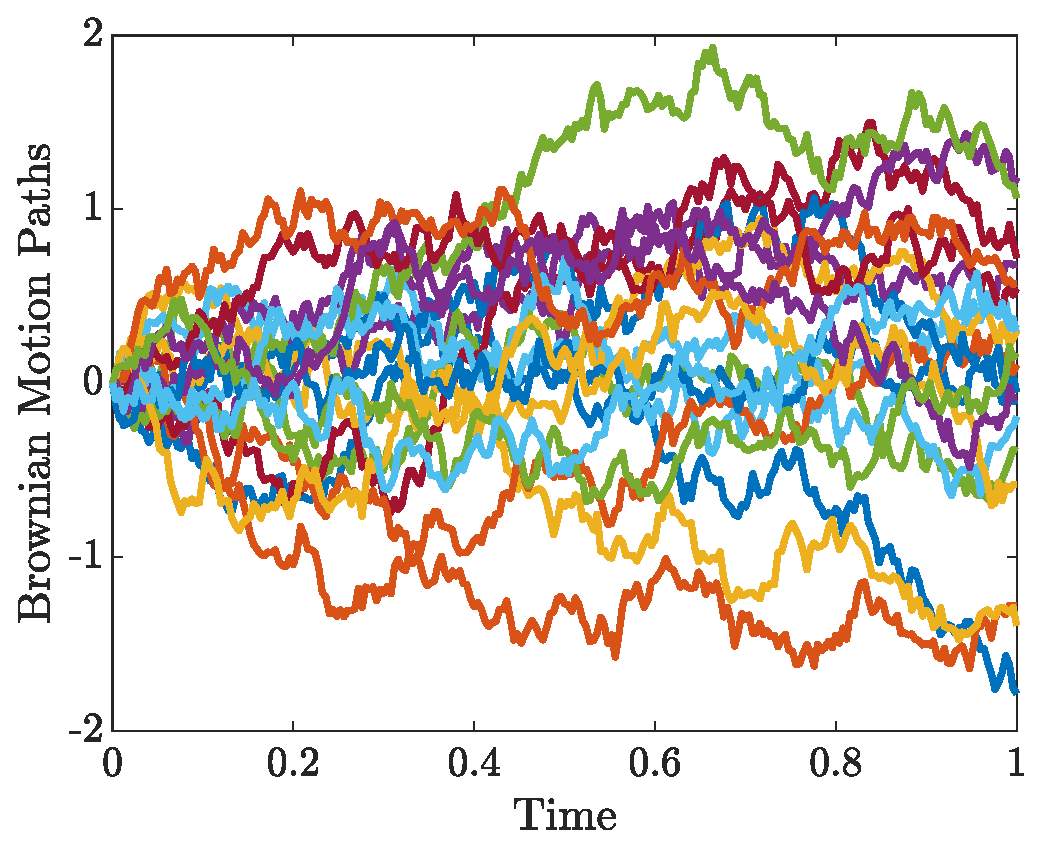
\includegraphics[scale =  0.2 ]{BrownianMotionPaths.eps}
    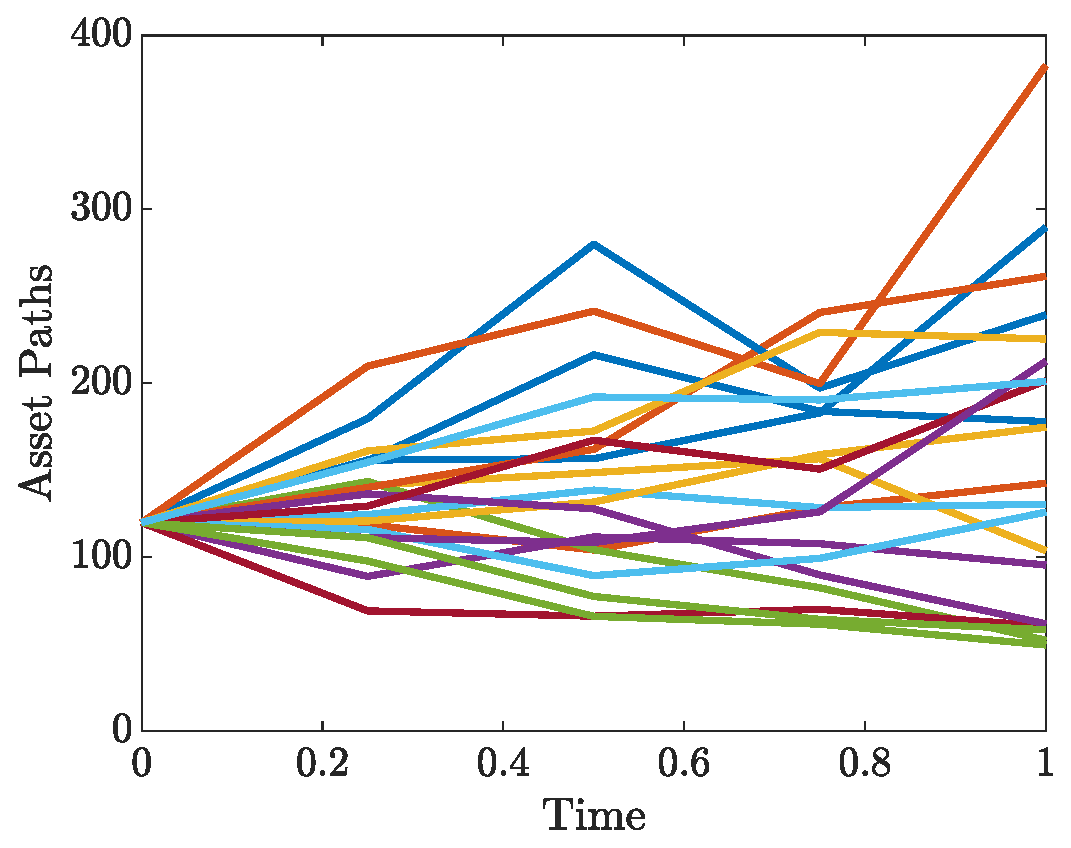
\includegraphics[scale =  0.2]{AssetPaths.eps}
    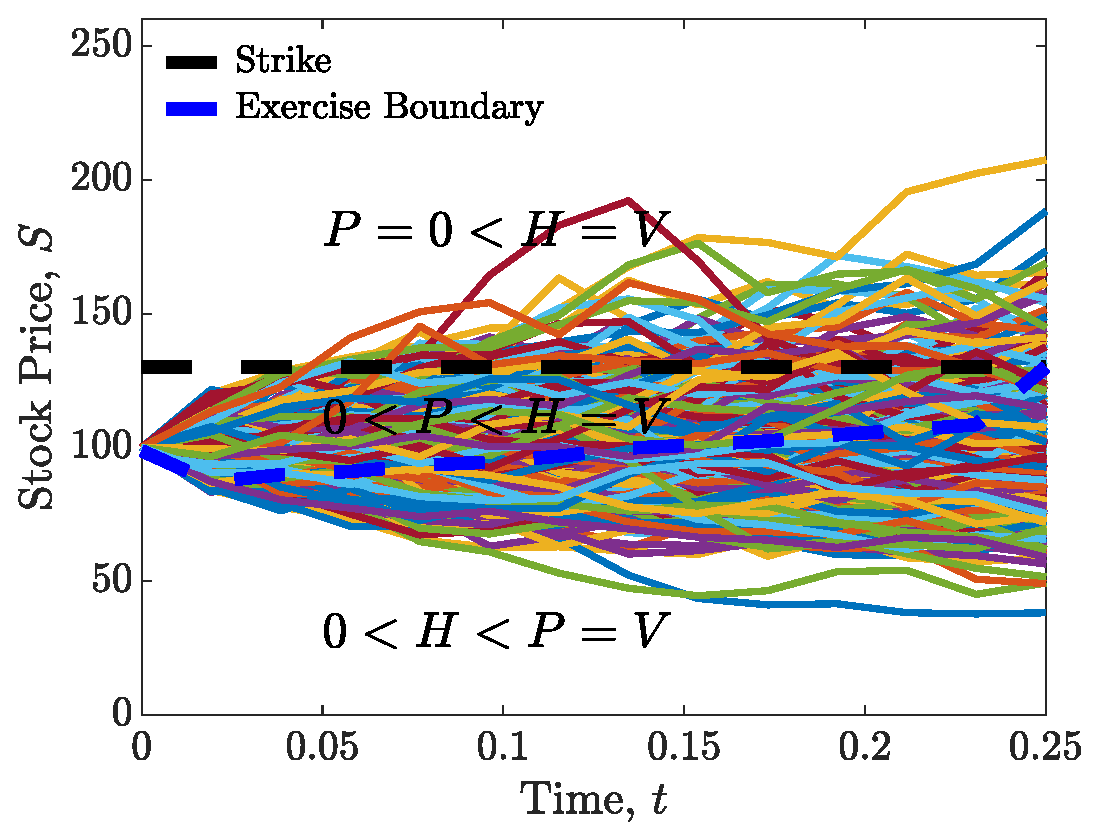
\includegraphics[scale =  0.2]{AmerPutPathsExer.eps} 
  \end{center}
  \caption{Brownian Motion; Asset Paths; Exercise Boundary}
  \label{fig:bmandassetpath}
\end{wrapfigure}


In this project, we focus on American options. Unlike European or Asian exercised options, which are exercised only at the expiry of the contract, American options may be exercised at any time during the contract. This flexibility makes pricing American options more difficult. The price of the option should depend on the option holder making the optimal exercise decision. However, the optimal exercise decision is not just as soon as one gets in the money or the time that maximizes the payoff over the life of the option because no one can know the future.

The optimal exercise decision is when the \emph{discounted payoff from exercising first exceeds the expected discounted value of continuing to hold the option}, see the third figure of Figure \ref{fig:bmandassetpath}, where $P$ is the discounted payoff, $H$ is the expected discounted holding value, and $V$ is the discounted value of the option and $V = \max\{P,H\}$. The expected discounted holding value $H$ must be computed at discrete times backwards by a biased-low method proposed by
Longstaff and Schwartz \cite{LonSch01}.
Instead of using Monte Carlo methods or quasi-Monte Carlo methods, we will consider to use the randomized quasi-Monte Carlo (RQMC) given by Pierre L'Ecuyer in the invited tutorial in the conference of Monte Carlo and quasi-Monte Carlo in 2016 \cite{RQMC}. A tool to generate the RQMC point sets was presented in 2020 \cite{toolforRQMC}. 



SURE students will learn how to generate BM and asset paths from RQMC point sets, construct the least squares regression method to obtain the decision boundary, and finally get the price estimation of the option. The results and computational time costs will be compared with those generated from QMC point sets. In addition, they will investigate other methods to increase the efficiency in pricing American options, such as control variates and importance sampling  \cite{NickiCV,ISref1,ISref2,ISref3}. Numerical experiments will be conducted to find an optimal way to price American options.








